\section{Overall description}
The purpose of this section is to provide a brief description of the project and to describe known actors and their interaction with the system. The section presents a high level view. For more detailed information, please refer to the developer team.

	\subsection{Stakeholders}
	\begin{itemize}
		\item \textbf{Rowing club administrators:} Must integrate the system into the rowing club's network infrastructure. Their concern is, that the system is usable for logging routes without any extended knowledge of computer systems.
		\item \textbf{Developers:} JEE course students, that are developing the system. Developers include architects, testers and quality engineers.
		\item \textbf{Rowing club members:} Use the system to log their rowed routes.
		\item \textbf{Lecturer:} Checks the state of development and marks the result of the developers for the JEE course.
	\end{itemize}
	
	\subsection{Actors}
	The following actors can be defined:\\
	
	\begin{itemize}
		\item \textbf{Rowing club administrator:} The rowing club administrator uses the system to create and publish boats and routes. Rowing club administrators also use the system to generate analysis and view statistics. Another task of him is to observe the status of boats for retrieving information about damaged boats.
		\item \textbf{Rowing club member:} The rowing club member uses the system to log their rowed routes and publish these routes on their profile.
	\end{itemize}
	
	
	\subsection{Use case Model Survey}
	According to the four parts identified in section \ref{scope}, the use case model is broken into packages. The use cases presented in this survey are high level use cases and are presented in figure \ref{img:rowbuddyPackages}.
	
	\begin{figure}[h!]
		\begin{center}
			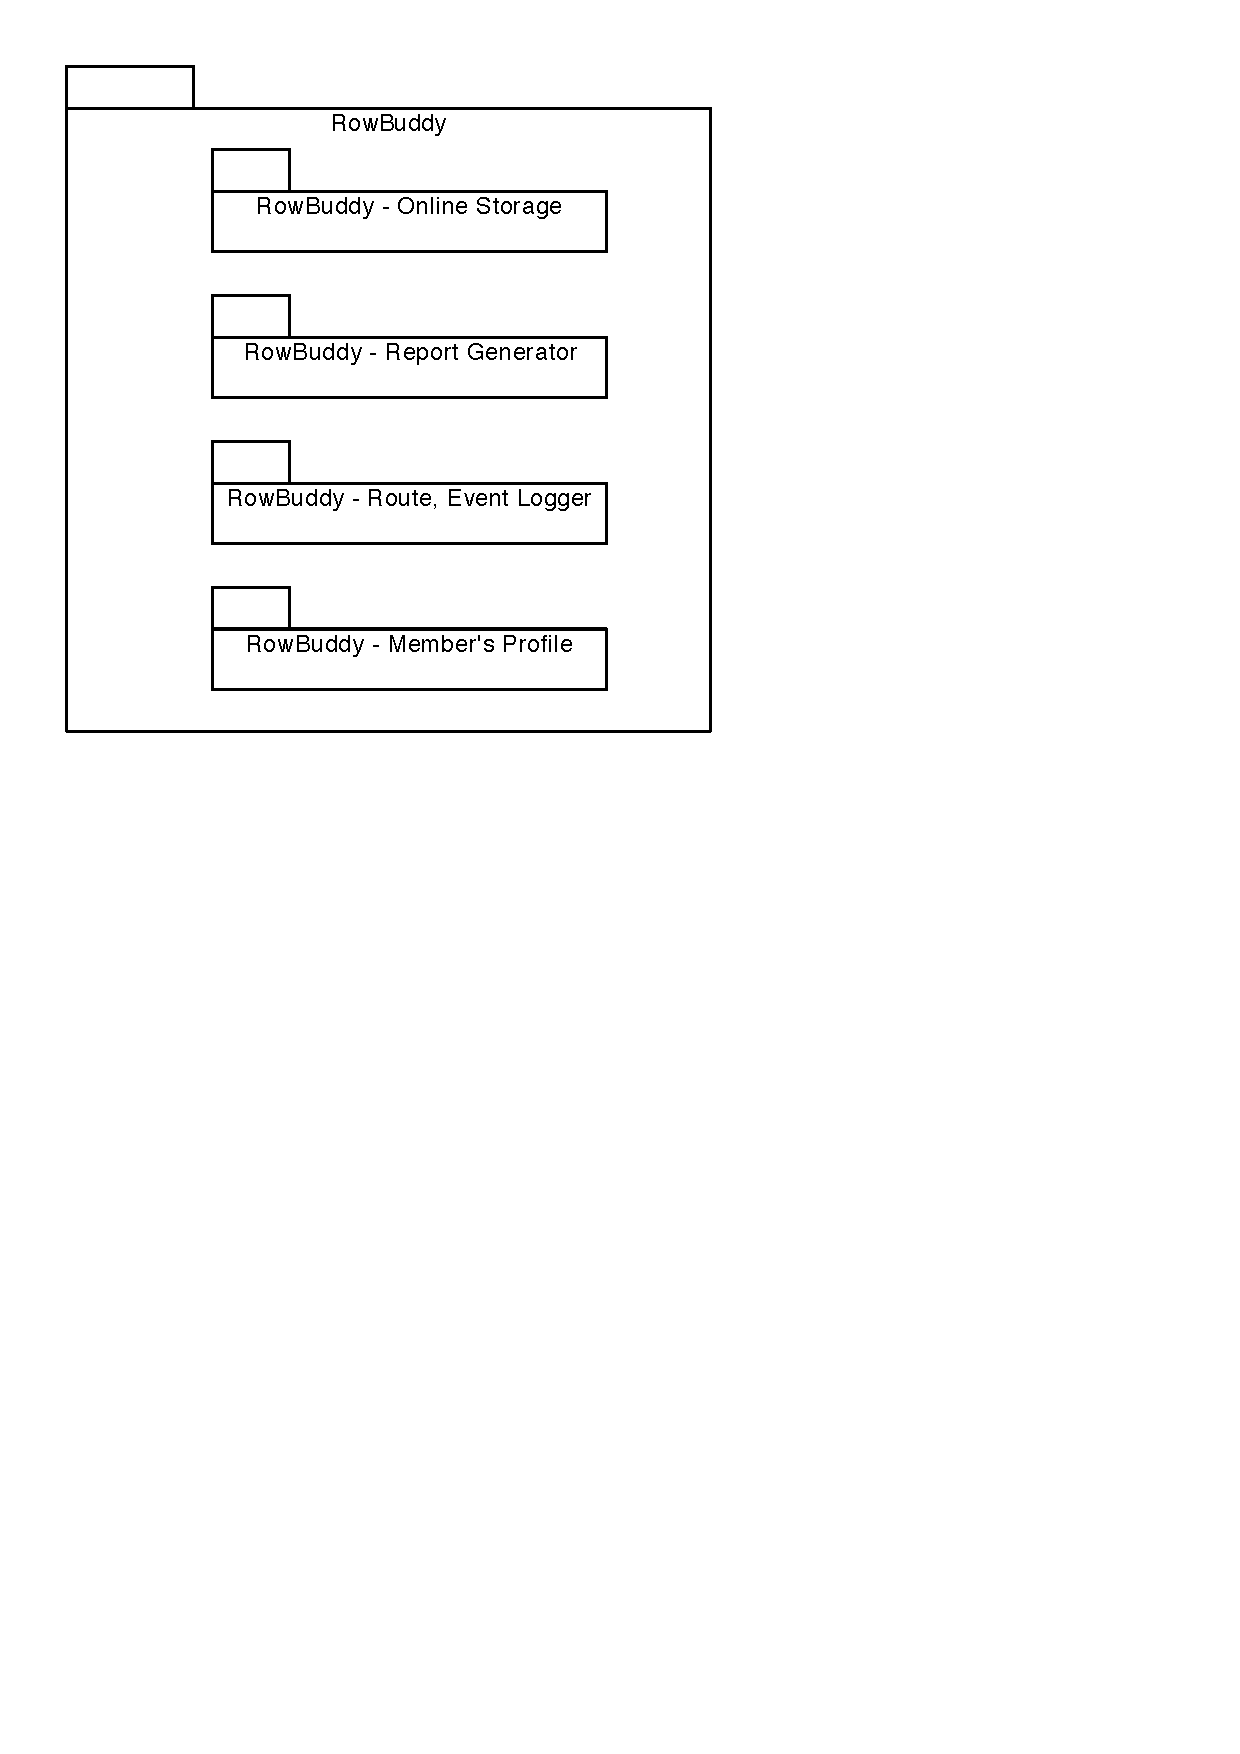
\includegraphics[width=0.5\textwidth]{./figures/rowbuddy_packages.pdf}
			\caption{RowBuddy Packages}
			\label{img:rowbuddyPackages}
		\end{center}
	\end{figure}
	
	
	
		\subsubsection{Package RowBuddy Online Storage}
		The use cases in the \textit{RowBuddy Online Storage package} deal with configuring, setting up and using the system as an administrator.\\

\hluc{HLUC-1}{Manage Boats}{RowBuddy Online Storage}{1}{wal}{}{%
		In this use case the Manager configures boats. It includes adding, removing, browsing and locking a boat if it is damaged.
The user can select a free boat for the next tour.	
		}	

\hluc{HLUC-2}{Manage Users/Accounts}{RowBuddy Online Storage}{1}{wal}{}{%
		In this use case the Manager configures users, user rights and accounts. Users
are members of the club. The user will automatically receive an account when they sign up in the club. This requires that an e-mail address is provided. The administrator also need additional functions within their user account.
This use case includes adding, browsing, changing, removing users and creating and removing accounts.	
		}

\hluc{HLUC-3}{Manage Routes}{RowBuddy Online Storage}{1}{wal}{}{%
		In this use case the Users configures routes. It includes adding, removing, browsing and changing routes. A route contains a name and description.
		}
		
		
		\subsubsection{Package RowBuddy Route and Event Logger}
		The use cases in the \textit{RowBuddy Route and Event Logger package} deal with logging new routes and other things. Users may p.e. log a damaged boat.\\
		
		TODO IMAGE
		\begin{itemize}
			\item \textbf{HLUC-4:} Log rowed route
			\item \textbf{HLUC-5:} Log damaged boat
		\end{itemize}
		
		\subsubsection{Package RowBuddy Report Generator}
		The use cases in the \textit{RowBuddy Report Generator package} deal with generating all kinds of reports. The content of the reports are configurable to individualize the reports based on the logged routes.\\

		\hluc{HLUC-6}{Generate year statistic of all members}{ RowBuddy Report Generator}{1}{dch and wal}{}{%
		
		In this use case the Manager can create a report and statistic of all members. - Or - In this use case the program automatically create a statistic of all members every year. The Manager can set a specific date when it should create the statistics. The statistic contains information about the most valuable rower, most improved rower, graphical representation and best rookies. This use case also include browsing and creating statistics. The members are able to see the generated statistics.
		}

\hluc{HLUC-7}{Generate boat statistics}{ RowBuddy Report Generator}{1}{wal}{}{%
		In this use case the Manager can create a report and statistic of all boats. - Or - In this use case the programm automatically create a statistic of all boats. The Manager can set a specific date when it should create the statistics. This statistic includes new boats, broken boats and boats are no longer used. The users can see this statistic. This use case includes browsing and creating statistics.
		}

\hluc{HLUC-8}{Generate individual statistics for a member}{ RowBuddy Report Generator}{1}{dch}{}{%
		Each member has an own personal statistic about his activities. This statistic is generated on demand by the member itself. The statistic is attached to the users profile and contains information about total distance, popular routes and used boats.
		}
		
		\subsubsection{Package RowBuddy Member's Profile}
		The use cases in the \textit{RowBuddy Member's Profile package} deal with the profiles of a member. How he can publish his own results and how to view the profiles of other row buddys.\\
		
		TODO IMAGE
		\begin{itemize}
			\item \textbf{HLUC-9:} Publish route on profile
			\item \textbf{HLUC-10:} View other club members profile
			\item \textbf{HLUC-11:} Login user
		\end{itemize}
		
		
		\hluc{HLUC-1}{Add Pattern}{Pattern Management}{1}{jnt}{\nameref{scope}}{%
		lorem ipsum\newline	
		}
		